\documentclass{udparticle}
\setlogo{EIT}
\headertext{Respuestas tarea de preparación para la Solemne }
\title{Tarea de preparación para la Solemne 2}
\author{Ignacio Yanjari, Dagoberto Navarrete, Ignacio López, Thomas Muñoz.}
\usepackage{graphicx}
\usepackage{float}
\graphicspath{ {images/} }
\begin{document}
\maketitle
\begin{enumerate}
%\clearpage
\item Nombre 3 servicios ofrecidos por la Capa de RED.
\begin{enumerate}
\item Permite la conexión entre 2 redes geograficamente distintas
\item Busca la mejor ruta desde una red a otra mediante criterios
\item Utiliza un sistema de correccion de errores al transportar paquetes
\end{enumerate}
\item Explique brevemente las causas que gatillaron el problema de escases de las direcciones IPv4.\\
Mencione 3 mecanismos utilizados actualmente para mitigar este problema.\\\\
Como solo existian Clases de IPs con mascaras por defecto para c/clase,generaba una 
perdida de muchas combinaciones de ip al momento de asignarle una clase a una casa por 
ejemplo.\\
Mecanismos para mitigar problemática:
\begin{enumerate}
\item Tecnica de sumarizacion de redes 
\item Tecnica de  creacion de subredes
\item Ip privada y Ip pública
\end{enumerate}
\item Realice una breve descripción de cada uno de los campos de la cabecera IPv4. Se pide utilizar la aplicacion Wireshark para realizar 1 captura (pantallazo) e interpretar la información relacionada con la capa de red (todos los campos de la cabecera IPv4).
\item Explique las diferencias existentes entre el protocolo IPv4 e IPv6.
\begin{itemize}
	\item El protocolo IPv6 ofrece una mayor cantidad de direcciones que IPv4.
	\item El protocolo IPv4 está basada en 32 bits, en cambio IPv6 está basado en 128 bits.
	\item El protocolo IPv4 tiene una representación decimal a diferencia de IPv6 que su representación es hexadecimal.
\end{itemize}
\item El prefijo de una red IPv6 es: 2001:0720:1014:0002. Se conecta un
computador cuya dirección física MAC es 0008:0267:5CCA. Se pide indicar la direccion IPv6 del equipo.
\item ¿Cual es la unidad máxima de transferencia MTU para una red Ethernet?
	1500 bytes.
\item Indique la dirección resumida de la IPv6 0004:0000:0000:0000:000A:0000:0000:1243:00AD
	4::A::1243:AD
\item Explique las diferencias existentes entre los modos túnel, traductor y dual stack
\begin{itemize}
	\item {\bf Modo túnel}: Se utilizan túneles encapsulando IPv6 dentro de IPv4, permitiendo de esta forma atravesar redes que no manejan IPv6, pero también podemos encontrar la situación inversa. En síntesis los paquetes originales son transportados hasta un punto de la red por medio del protocolo original, luego encapsulados para atravesar la porción de red que no lo soporta y luego des-encapsulados en el otro extremo para ser enviados al destino final en su forma original.
	\item {\bf Modo traductor}: Esta técnica consiste en utilizar algún dispositivo en la red que convierta los paquetes de IPv4 a IPv6 y viceversa. Ese dispositivo tiene que ser capaz de realizar la traducción en los dos sentidos de forma de permitir la comunicación.
	\item {\bf Dual Stack}: Por este método un host o un router tendrán ambas pilas de protocolos, IPv4 e IPv6. Por consiguiente las dos pilas envían y reciben datagramas que pertenecen a ambos protocolos y así podrán comunicarse con cada nodo IPv4 e IPv6 en la red.
\end{itemize}
\clearpage
\item Se pide realizar la conversión binaria a decimal de la información contenida en la tabla Figura 1.
	\begin{figure}[H]
	\centering
	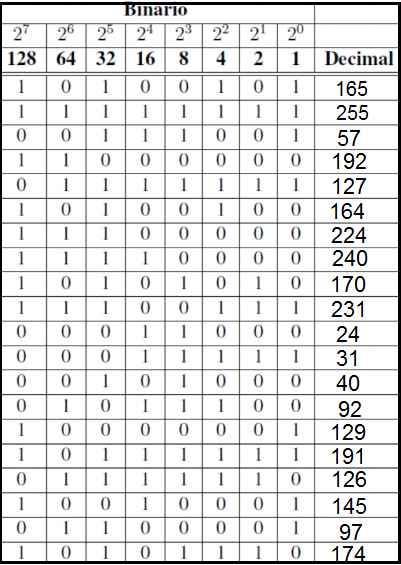
\includegraphics[width=15cm]{fig1}
	\caption{Cálculo de binario a decimal}
	\end{figure}
\clearpage

\item Se pide realizar la conversion de decimal a binario de la información contenida en la tabla de la Figura 2.
	\begin{figure}[H]
	\centering
	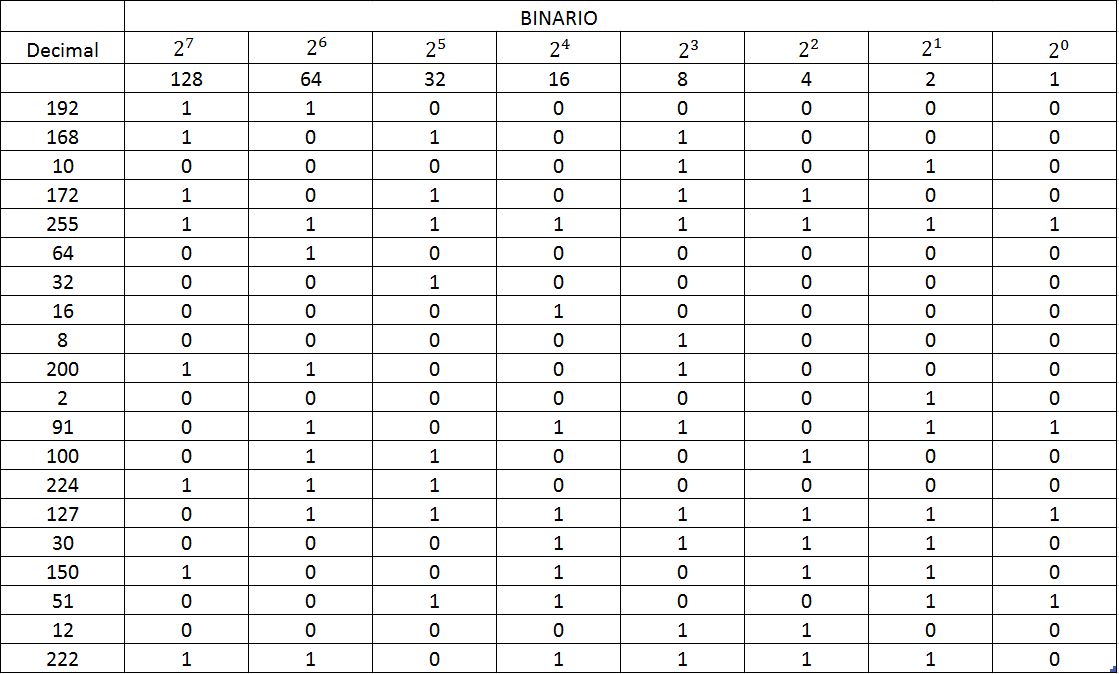
\includegraphics[width=15cm]{fig2}
	\caption{Cálculo de decimal a binario}
	\end{figure}

%insertar figura 2
\item Indique la importancia del uso de NAT/PAT.\\\\
Permite el uso de ip privadas y publicas.Siendo privadas las que se encuentran en la LAN y las ip pública es la
salida de esta LAN recien mencionada a la WAN.Generando asi menor cantidad de ips en uso ya que pueden existir
2 ips iguales pero dentro de difentes LAN.
\item ¿Que es NAT? ¿Qué es PAT?\\\\
Son tipos de traducciones dentro de un router :
\begin{enumerate}
	\item NAT : genera la asociación entre una IP pública y una IP privada dentro de la red
	\item PAT : genera la asociación entre una Ip pública con su respectivo puerto en el router
\end{enumerate}
\item Explique las diferencias entre NAT estática y NAT dinámica.
\begin{enumerate}
\item NAT estática es una traducción sin cambios automáticos,dejando a el administrador como
el que configure la tabla.Esto se aplica principalmente para dispositivos que como requerimiento
necesiten una IP estática,por ejemplo Servidor WEB.Si se quisieran agregar más servidores se tendrían que 
configurar todos manualmente.\\
\item NAT dinámica es una traducción en la cual cuando se agrega un dispositivo en la LAN, automáticamente
se configura la tabla sin necesidad de un administrador.Se usa para host como PC,ya que estos pueden utilizar
IP dinámica y así se facilitaria la conección de una gran cantidad de dispositivos.\\
\end{enumerate}
\item Un router que hace la siguiente NAT dinamica: red interior 
192.168.0.0/24 <=> red exterior 200.230.16.192/26.\\
¿Cual es el rango de direcciones IPs pública con los que los equipos 
pueden salir?
\item ¿Que es una ACL estándar?\\\\
Una ACL es una lista de control de acceso permitida en los routers,el tipo estándar permite filtrar antes o despues 
de pasar por el router pero solo se puede filtrar según IP origen.ubicando en la wild-card el 0 indica el valor estático 
y 1 el variable.\\
por ejemplo:
\begin{enumerate}
\item para filtrar un solo usuario de ip 192.13.13.1 se ocuparia la wild-card igual a 0.0.0.0
\item para filtrar una red de ip 192.13.13.0 se le aplicaría la wild-card igual a 0.0.0.255
\end{enumerate}
Sintaxis ''Router (config-if)# ip access-group nº in|out"
\item ¿Que es una ACL extendida?\\\\
Una ACL es una lista de control de acceso 
permitida en los routers,el tipo extendida 
permite filtrar antes o despues
dependiendo de el protocolo(IP, ICMP, TCP, 
UDP, ...)tendremos opciones de 
configuración diferente, siempre acorde con
el protocolo, es decir con TCP podré 
utilizar operación de puertos pero con IP 
no.\\\\
sintaxis 'Router (config)# access-list nº 
permit|deny protocolo origen [wild-mask] [operación] [puerto origen] destino [wild-mask] [operación] [puerto destino] [established]"

\item La empresa ACME SA tiene una red como la que muestra la siguiente Figura . 
En el router R0 se han establecido 2 ACLs. La primera ACL tiene por 
objetivo de filtrar el tráfico de entrada hacia el 
servidor DMZ con las siguientes reglas:\\
Regla1 > permit tcp any any\\
Regla2 > permit udp any any\\
Regla3 > permit ip any any\\
Regla4 > permit icmp any any\\
La segunda ACL filtra el trafico de entrada hacia la red 
192.168.1.0/24:\\
Regla1 > deny tcp any 192.168.1.200\\
Regla2 > permit tcp any any\\
Regla3 > permit ip any 192.168.1.200\\
Regla4 > permit ip any any\\
Explique la funcion que cumple cada una de estas reglas.\\
\includegraphics[width=10cm]{fig3}\\
Filtrado Servidor DMZ
\begin{enumerate}
\item Las reglas 1-2-3-4 en el  permiten el ingreso de paquetes del tipo tcp,udo,ip,icmp provenientes de cualquier red y destino cualquiera dentro de la red
\end{enumerate}
Filtrado de entrada hacia la red 192.168.1.0/24
\begin{enumerate}
\item La regla 2-4 permiten el ingreso de paquetes del tipo tcp,ip de origen y destino cualquiera sea éste
\item La regla 3 permite el ingreso de paquetes del tipo ip con destino 192.168.1.200
\item La regla 1 niega el ingreso de paquetes del tipo tcp con destino  192.168.1.200
\end{enumerate}
\item Implemente los filtros necesarios para controlar los posibles ataques a los equipos de la red ACME, excepto los que corresponden
a los servicios web y ftp que se encuentran alojados en el servidor 192.168.1.200.\\

\item ¿Que es una subred?.\\\\
Es una division de una red cuando estás 
son muy grandes. Sirve para reducir el 
dominio broadcast y obtener un mayor 
manejo dentro
de la red.
\item De la direccion de red 136.228.0.0 se han de generar 99 subredes de igual tamaño.¿Cuál es la máscara que se debe utilizar?.\\\\
La máscara a utilizar para cada subred debe ser de 255.255.255.128
ya que para generar al menos 99 subredes se necesita ocupar 
\[2^7=128\]
con la cual incluso se podrían crear 29 subredes más 
\item Para la misma red del caso anterior, indique la cantidad máxima de hosts que por cada una de las subredes\\\\
La cantidad máxima de host está dado por la formula
como la máscara usada en el caso anterior es de tipo 255.255.255.128 y la cantidad de host posibles sería 
\[2^7-2=126\]
\item Si se tiene un host cuya direccion IP y prefijo son: 19.95.99.210/25. Indique su dirección de red.\\\\
Su dirección de red es 19.95.99.210 (nombre de la red)
\item Si una red Clase C se divide en subredes cuya mascara es
255.255.255.192, ¿Cuántas subredes utilizables se crean?.\\\\
la mascara de las subredes de la forma 255.255.255.192 ocupa 
26 bits para nombre de la red dejando 6 bits para host.Como la  %tiene 62 host
clase C tiene una mascara de tipo 255.255.255.0 se pueden crear
\[2^2=4\]
subredes de mascara 255.255.255.192.
%Clase C: 192.168.0.0 a 192.168.255.255 (24 bits red, 8 bits hosts)
\item Dada una dirección IP de host 192.168.5.121 y una máscara de 
subred 255.255.255.248, ¿Cuál es el numero IP de la red del host?.

\item ¿En que se diferencian las direcciones de MAC de las de la capa de red?.
Las direcciones MAC están dadas por la tarjeta de red del equipo, son estáticas (no cambian) y permiten que equipos dentro de la misma red se comuniquen entre si, en cambio las direcciones de la capa de red (direcciones IP) son configurables y pueden ser dinámicas y permiten que los equipos se comuniquen con otros en otra red.
\item ¿Cuantas direcciones útiles de host se pueden utilizar en una red con prefijo 24?.\\\\
Se pueden agregar \[2^7=255\]
luego se le quitan 2 ips ,una para el nombre de la red  y otra para el 
broadcast, por lo tanto quedan 254 ips libres para host
\item ¿Cuantas subredes pueden tener una red que tiene un prefijo 16?.
	65536 subredes y 65534 subredes utilizables % revisar esta !!
\item ¿Cual es el número mínimo de bits que se pueden tomar prestados para formar una subred?.\\\\
El mínimo de bits que se necesitan para formar una subred son 2, ya que se necesitan 2 direcciones IP para host, una para la dirección de la red y una para el  broadcast de la red, dando una cantidad de 4 IPs, las cuales se pueden obtener utilizando 2 bits.
\item ¿Cuales son las principales razones para utilizar subredes?.\\\\
Las principales razones son:
\begin{enumerate}
\item Reduce el dominio broadcast.
\item Separar tipos de usuarios.
\item Optimiza la cantidad de IPs usadas en cada red.
\item Mejora la seguridad.
\item Control de acceso(ACL).
\end{enumerate}
\item Al realizar una operacion booleana en las direcciones IP 
131.8.2.5 AND 255.0.0.0 como lo haría un router, ¿Cuál sería la 
dirección de red/subred?.\\\\
sería 131.0.0.0 ya que la operacion AND se define como:
\begin{enumerate}
\item 1 AND 1 = 1
\item 0 AND 1 = 0
\item 1 AND 0 = 0
\item 0 AND 0 = 0
\end{enumerate}

\item Con una direccion de Clase C de 197.15.22.31 y una máscara de red
de 255.255.255.224,¿cuántos bits se tienen que tomar prestados para 
crear subredes?.\\\\
la mascara de red 255.255.255.224 ocupa 5 bits para host y 27 bits para la dirección de  red.\\
Ahora las direcciones de clase C ocupan 8 bits para host y 24 bits para nombre de la red.\\
Por lo tanto se utilizan 3 bits para generar subredes de máscara 255.255.255.224
\item Si usted quiere tener 12 subredes de Clase C, ¿cual es 
la máscara a utilizar?.
\item Si usted necesita una red de prefijo 16 y desea generar 
510 direcciones de subredes, ¿cuál es la máscara que se deber 
ıa utilizar?.
\item De la topología de red, mostrada en la siguiente Figura , se deben generar
las subredes solicitadas, para esto usted debe utilizar la tecnica de 
longitud de máscara variable VLSM de tal forma de maximizar el 
espacio de direcciones IPs. Se dispone de la dirección 
192.200.254.0/23 la cual usted debe utilizar para generar las 
subredes. Se pide completar la tabla de la Figura 5. Nota: las 
direcciones IP de las interfaces FastEthernet de todos los routers NO están consideradas en los requerimientos.\\
\includegraphics[width=15cm]{fig4}
\\\\\\
Respuesta :\\
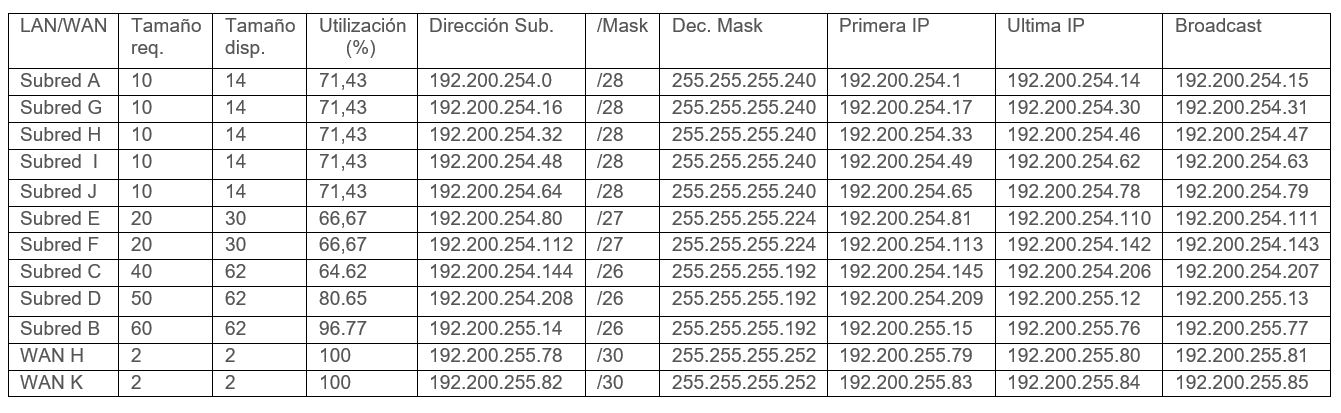
\includegraphics[width=15cm]{Ejercicio34}

\item Usted, como especialista en el diseno de redes LAN, ha sido seleccionado para
finalizar el proyecto que se muestra en siguiente  Figura . El ISP le ha asignado 2 
direcciones IP publicas: la dirección 177.12.180.252/30, que será utilizada como 
enlace con el ISP, y la dirección 200.198.248.0/21 la cual debe utilizar para generar las subredes necesarias mediante la técnica de máscara variable VLSM.
Se pide completar el diagrama de red (Figura 6) con la informacion solicitada
(direcciones de sub-redes, máscaras, dirección de broadcast, dirección IP 
hosts, gateway y enlaces seriales).
\includegraphics[width=15cm]{fig6}
%Insertar figura 6
\item Una organizacion se divide en dos departamentos A y B. La red corporativa de 
dicha organización se divide, a su vez, en cinco subredes tal y como muestra la siguiente
Figura . Para ello, la organizacion dispone de la dirección de red 138.8.0.0. 
Las subredes A1, A2 y A3 pertenecen al departamento A, y las subredes B1 y B2 
pertenecen al departamento B. Dicha red corporativa se conecta a Internet    a traves 
del router 3.
\begin{enumerate}
\item ¿Que máscara de red se debe utilizar en cada una de las redes en que se ha dividido la red corporativa original, si se desea que quede asignable en 
cada una de dichas redes el mayor numero posible de direcciones IP?
\item¿Cual es el máximo número de direcciones IP asignables a cada una de las subredes?
\item ¿Que dirección IP destino debe utilizar un equipo perteneciente a la 
subred B2 si desea transferir un paquete IP a todos los equipos de la red 
A2?
\item ¿Podría transferir, un equipo perteneciente a la subred B1, un paquete 
IP a todos los equipos del departamento A?. En caso de que la respuesta sea afirmativa,indique que dirección IP de destino se debe utilizar\\
\end{enumerate}
\includegraphics[width=15cm]{fig7}
\item De la topología de red de la siguiente Figura , complete la tabla de rutas del 
Router/Firewall. Indique si es posible realizar una sumarización de la tabla 
de rutas anterior (justifique). Si su respuesta es afirmativa se pide
construir esta tabla de rutas resumida.
	\begin{figure}[H]
	\centering
	\includegraphics[width=15cm]{fig8}
	\end{figure}
%insertar figura 8
\item Dada la siguiente topología de la siguiente Figura , encontrar la tabla de rutas 
del router R1. También se pide encontrar la tabla de ruta sumarizada. En 
ambos casos considere la existencia de una ruta por defecto.
	\begin{figure}[H]
	\centering
	\includegraphics[width=15cm]{fig9}
	\end{figure}
\item Se tiene la siguiente tabla (Figura siguiente) de enrutamiento sin CIDR. Encuentre 
la tabla del router reducida utilizando sumarizacion CIDR.
	\begin{figure}[H]
	\centering
	\includegraphics[width=15cm]{fig10}
	\end{figure}
%Insertar figura 10
\item En la red de la siguiente Figura  las redes Ethernet conectadas a R1 han sido 
notificadas de manera sumarizada hacia R2 como 192.168.144.0/20. ¿Cuáles serán 
las direcciones IP de los paquetes que se enviara el router R2 hacia R1, de acuerdo a este resumen?.
	\begin{figure}[H]
	\centering
	\includegraphics[width=15cm]{fig11}

	\end{figure}
%Insertar figura 11
\item Para la red de la siguiente Figura , determine, ¿cuál es la mejor ruta sumarizada que
enviará R3 a R4?.
	\begin{figure}[H]
	\centering
	\includegraphics[width=15cm]{fig12}
	\end{figure}
%Insertar figura 12

\item Para la red de la Figura siguiente , determine si el usuario de notebook del 
departamento de VENTAS de la SUCURSAL 1 puede o no puede comunicarse con el Server 
A del departamento de MARKETING,ubicado en la CASA MATRIZ. Si su respuesta es 
negativa, indique cómo resolver el problema.
	\begin{figure}[H]
	\centering
	\includegraphics[width=15cm]{fig13}
	\end{figure}

\item Después de ser instalada y configurada la red de la Figura siguiente, se ha 
comprobado que ésta no funciona correctamente. Usted, como especialista, ha sido 
contratado para resolver el problema. Identifique el problema y proponga el o los 
cambios que se deben realizar.
	\begin{figure}[H]
	\centering
	\includegraphics[width=15cm]{fig14}
	\end{figure}
\item Nombre 3 servicios ofrecidos por la capa de Transporte.
\begin{enumerate}
\item Seguridad 
\item Confiabilidad
\item Buena conección entre Usuruario-Servidor
\end{enumerate}
\end{enumerate}
\end{document}
